\section{Numerical experiments}\label{sec:numerical_experiments}

We evaluate PFAOS and MC-PFAOS on monotone variational inequalities arising
from bilinear games with convex quadratic coupling constraints. The
experiments address three questions. First, how do the proposed methods
perform when neither the operator Lipschitz constant nor the constraint
smoothness constants are available to their line searches? Second, how
does their computational effort compare with operator extrapolation (OE)
when each OE step requires projection onto the complete nonlinear feasible
set? Third, how does this comparison change with the dimension of the game
and the number of coupling constraints? We examine these questions through
two experiments: a comparison of PFAOS and projected OE with one constraint,
and a comparison of MC-PFAOS and projected OE with multiple constraints.
Each comparison uses the same realized instance and the same initial point.

\subsection{Generation of structured test instances}\label{subsec:numerical_instances}

We construct a bilinear game with a singular positive semidefinite regularizer,
making its VI operator monotone but not strongly monotone, and choose the
quadratic resource limits so the compact convex feasible set contains a
strictly feasible point and admits a solution. We bound the operator's scale
and rescale each resource constraint by $m^{-1/2}$ to keep comparisons across
$n$ and $m$ meaningful, while retaining the bilinear interaction and nonlinear
coupling that make the instances nontrivial.

\paragraph{Game structure and operator normalization.}
Let $x=(u,v)\in\mathbb R^n$, where
$u\in\mathbb R^{p}$, $v\in\mathbb R^{q}$,
$p=\lfloor n/2\rfloor$, and $q=n-p$. The two players minimize and maximize,
respectively, the regularized bilinear payoff
\begin{equation}\label{eq:numerical_game}
\Phi(u,v)=u^\top Cv+\frac12u^\top H_u u
-\frac12v^\top H_v v-d_u^\top u+d_v^\top v.
\end{equation}
The associated variational inequality operator is
\begin{equation}\label{eq:numerical_operator}
\begin{aligned}
F(x)&=Bx-d
=\begin{pmatrix}H_u u+Cv-d_u\\ H_vv-C^\top u-d_v\end{pmatrix},\\
B&=S+H,\qquad
S=\begin{pmatrix}0&C\\-C^\top&0\end{pmatrix},\qquad
H=\operatorname{Diag}(H_u,H_v),\qquad d=(d_u,d_v).
\end{aligned}
\end{equation}
Thus $F=(\nabla_u\Phi,-\nabla_v\Phi)$. The players share the base set
$X=\{x\in\mathbb R^n:\|x\|_2\le r\}$ and the resource constraints
defined below, with $r=1$ throughout. Because these restrictions couple the
players' decisions, we solve the variational equilibrium formulation on
their common feasible set. This construction gives the instances a
continuous-strategy game interpretation, with a bilinear interaction and
convex--concave quadratic regularization.

The payoff matrix $C\in\mathbb R^{p\times q}$ is sparse, with entries
$C_{j,j}=0.7$, $C_{j,j+1}=0.15$, and $C_{j+1,j}=-0.15$ whenever the
corresponding indices are valid; all other entries are zero. To generate
$H$, we draw its diagonal entries from $\mathrm{Unif}(0.1,0.4)$ and set
entries $1,4,7,\ldots$ to zero. The blocks $H_u$ and $H_v$ are the first
$p$ and last $q$ coordinates of this diagonal matrix. We draw a standard
Gaussian vector $\widetilde d$ and set
$d=\widetilde d/\|\widetilde d\|_2$.
The symmetric part of $B$ is therefore the singular positive semidefinite
matrix $H$, so $F$ is monotone but not strongly monotone. Moreover,
$\|C\|_2\le1$, $\|H\|_2\le0.4$, and
\[
L_F=\|B\|_2\le1.4,\qquad \|d\|_2=1.
\]
These bounds keep the operator scale comparable across dimensions. The
sparse representation also allows an evaluation of $F$ in $O(n)$ work,
without storing a dense $n\times n$ matrix. PFAOS and MC-PFAOS are not given
$L_F$ or its construction-based bound.

\paragraph{Shared resource constraints.}
For each instance, define the unscaled quadratic functions
\[
h_i(x)=\tfrac12x^\top A_i x+b_i^\top x+c_i
\]
and set
\begin{equation}\label{eq:numerical_quadratic_constraints}
g_i(x)=\frac{h_i(x)}{\sqrt m},\qquad
G(x)=(g_1(x),\ldots,g_m(x))^\top,\qquad
\widetilde X=\{x\in X:G(x)\le0\}.
\end{equation}
The matrices $A_i$ are diagonal and positive semidefinite. We construct
the constraints from five resource types so that increasing $m$ adds
related resource limits while keeping the underlying feasible geometry
broadly comparable. For type $t\in\{1,\ldots,5\}$ and coordinate
$j\in\{1,\ldots,n\}$, generate a mask
$\omega_{tj}\sim\mathrm{Bernoulli}(1/2)$ and a coefficient
$a_{tj}\sim\mathrm{Unif}(0.1,0.4)$. Also generate a unit vector $s_t$ by
normalizing a standard Gaussian vector. Constraint $i$ uses type
$t(i)=1+((i-1)\bmod 5)$ and has coefficients
\begin{equation}\label{eq:numerical_resource_coefficients}
\begin{aligned}
\bigl[A_i\bigr]_{jj}&=\omega_{t(i),j}a_{t(i),j}(1+\rho_{ij}),
&\rho_{ij}&\sim\mathrm{Unif}(-0.02,0.02),\\
b_i&=0.7d+0.5s_{t(i)}+0.01w_i,
&w_i&=\widetilde w_i/\|\widetilde w_i\|_2,
\end{aligned}
\end{equation}
where $j=1,\ldots,n$ and $\widetilde w_i$ is standard Gaussian. The type-specific masks,
coefficients, and directions are reused, while each constraint receives
its own perturbations. Every realized $A_i$ in the reported experiments
has at least one zero diagonal entry, and hence every constraint function
is convex but not strongly convex. The construction gives the uniform
bounds $\|A_i\|_2\le0.408$ and $\|b_i\|_2\le1.21$.

We choose the common initial point and the constraint offsets as
\begin{equation}\label{eq:numerical_slater_point}
x^{\mathrm f}=-0.35d,\qquad
c_i=-\frac12(x^{\mathrm f})^\top A_i x^{\mathrm f}
-b_i^\top x^{\mathrm f}-\delta,\qquad \delta=0.04.
\end{equation}
It follows that $\|x^{\mathrm f}\|_2=0.35<1$ and
$g_i(x^{\mathrm f})=-\delta/\sqrt m<0$ for every $i$. Thus the instances
have a common Slater point. In particular, $\widetilde X$ is nonempty,
compact, and convex; continuity and monotonicity of $F$ then ensure the
existence of a solution to the variational inequality. The same
construction is used for the single-constraint experiment ($m=1$) and the
multi-constraint experiment ($m\ge2$).

For these functions, the Jacobian and a valid vector smoothness constant
are
\begin{equation}\label{eq:numerical_constraint_smoothness}
J(x)=\frac{1}{\sqrt m}\begin{bmatrix}(A_1x+b_1)^\top\\ \vdots\\ (A_mx+b_m)^\top\end{bmatrix},
\qquad
L_G=\left(\frac1m\sum_{i=1}^m\|A_i\|_2^2\right)^{1/2}\le0.408.
\end{equation}
Indeed, for any $x,y\in X$,
\[
\|G(y)-G(x)-J(x)(y-x)\|_2
\le\frac{L_G}{2}\|y-x\|_2^2.
\]
When $m=1$, this reduces to the gradient smoothness constant
$L=\|A_1\|_2$. The factor $m^{-1/2}$ preserves the feasible set and
controls the scale of the vector constraint map as $m$ increases. It also
fixes the meaning of the reported feasibility measure:
\begin{equation}\label{eq:numerical_rms_violation}
\|[G(x)]_+\|_2
=\left(\frac1m\sum_{i=1}^m[h_i(x)]_+^2\right)^{1/2}.
\end{equation}
Thus comparisons across $m$ use the root-mean-square violation of the
unscaled resource limits. For fixed $n$ and seed, the operator, initial
point, and resource prototypes are held fixed as constraints are added.
The larger values of $m$ therefore represent additional, partly redundant
limits from the five types, rather than additional independent resource
types.

\subsection{Algorithms and projected-OE benchmark}
\label{subsec:numerical_methods}

\paragraph{PFAOS and MC-PFAOS.}
We implement Algorithms~\ref{alg:pfaos} and~\ref{alg:mc-pfaos} using their
prescribed averaging rules and line searches. PFAOS forms an affine model
of its single constraint and solves each primal subproblem by Euclidean
projection onto the intersection of $X$ and the resulting halfspace. This
projection is evaluated analytically by distinguishing which of the ball
and halfspace constraints are active. MC-PFAOS uses projection onto $X$
for its primal updates and componentwise projection onto
$\mathbb R_+^m$ for its dual updates, starting from $\lambda_0=0$.
Its primal updates therefore require no projection onto the polyhedron
defined by the linearized coupling constraints. Both methods start from
$x_0=x^{\mathrm f}$ and use $\Lambda=100$. This is the multiplier
parameter appearing in the algorithms and their analysis; it supplies no
Lipschitz or constraint-smoothness information.

We initialize constraint curvature from four pairs of local samples. For
$j=1,\ldots,4$, let
\[
u_j=0.25r\frac{a_j}{\|a_j\|_2},\qquad
v_j=0.75r\frac{e_j}{\|e_j\|_2},
\]
where $a_j$ and $e_j$ are independent standard Gaussian vectors. The
sampling stream uses the instance seed plus $10{,}000$. For PFAOS, the
sampled curvature is
\begin{equation}\label{eq:numerical_scalar_curvature}
\ell_j=
\frac{2\bigl(g(v_j)-g(u_j)
-\langle\nabla g(u_j),v_j-u_j\rangle\bigr)}
{\|v_j-u_j\|_2^2},
\end{equation}
where $g=g_1$. For MC-PFAOS, we use
\begin{equation}\label{eq:numerical_vector_curvature}
\ell_j=
\frac{2\|G(v_j)-G(u_j)-J(u_j)(v_j-u_j)\|_2}
{\|v_j-u_j\|_2^2}.
\end{equation}
In both cases, $L_0=0.5\max_{1\le j\le4}\ell_j$. The quotients are
bounded above by $L$ and $L_G$, respectively, and all sampled maxima in
the experiments are positive. The factor $0.5$ deliberately initializes
below the sampled curvature; the line searches subsequently determine
acceptable local estimates. We set the initial proximal and operator
parameters to $\eta_0=M_0=2\Lambda L_0$, as prescribed by the algorithms.
The four gradient or Jacobian evaluations and their sampling time are
included in the reported work and solver time. Numerical comparisons in
the proposed methods' line searches use a tolerance of $10^{-12}$, which
is distinct from the solution-accuracy target defined below.

\paragraph{Projected operator extrapolation.}
The benchmark applies OE to the original feasible set $\widetilde X$.
Set $x_{-1}=x_0=x^{\mathrm f}$. For each realized instance, let
$M=\|B\|_2$ and run OE with the three initial operator estimates
\[
\widehat M_0\in\{M,\ 0.1M,\ 10M\}.
\]
The spectral norm is computed to numerical precision before the timed runs.
These initializations isolate sensitivity to the operator estimate; neither
$L$ nor $L_G$ is an OE input because the nonlinear constraints are handled
by projection. The following operator line search is retained in all three
configurations. At iteration
$k\ge1$, trial $q\ge0$ is defined by
\begin{equation}\label{eq:numerical_projected_oe}
\begin{aligned}
\widehat M_k(q)&=2^q\widehat M_{k-1},\\
\theta_k(q)&=
\begin{cases}
1,&k=1,\\
\widehat M_k(q)/\widehat M_{k-1},&k\ge2,
\end{cases}\\
\widehat F_k(q)&=F(x_{k-1})
+\theta_k(q)\bigl(F(x_{k-1})-F(x_{k-2})\bigr),\\
x_k(q)&=\Pi_{\widetilde X}
\left(x_{k-1}-\frac{\widehat F_k(q)}{2\widehat M_k(q)}\right).
\end{aligned}
\end{equation}
We accept the first trial satisfying
\begin{equation}\label{eq:numerical_projected_oe_linesearch}
\|F(x_k(q))-F(x_{k-1})\|_2
\le\widehat M_k(q)\|x_k(q)-x_{k-1}\|_2,
\end{equation}
with a relative numerical allowance of order $10^{-12}$. If the test
fails, we increment $q$ and recompute the trial point, including its
projection. Writing $q_k$ for the accepted trial, we set
$\widehat M_k=\widehat M_k(q_k)$, $x_k=x_k(q_k)$, and report
$\bar x_k^{\mathrm{OE}}=k^{-1}\sum_{j=1}^k x_j$. Equivalently, each
accepted step minimizes
\[
\langle\widehat F_k(q_k),x\rangle
+\widehat M_k\|x-x_{k-1}\|_2^2
\quad\text{over }x\in\widetilde X.
\]
After initialization, the benchmark adapts its operator estimate from values
of $F$. The true operator norm is used only to define this controlled comparison
and is not supplied to either proposed method.

\paragraph{Generic nonlinear projection.}
For a trial center $z$, projected OE computes
\begin{equation}\label{eq:numerical_generic_projection}
\min_{x\in\mathbb R^n}\ \frac12\|x-z\|_2^2
\quad\text{subject to}\quad
\|x\|_2\le1,\qquad g_i(x)\le0,\quad i=1,\ldots,m.
\end{equation}
We model this convex problem in CVXPY and solve it with the general-purpose
Clarabel conic solver. Every trial, including one with an already feasible
center, constructs a new CVXPY problem containing all original quadratic
constraints and solves it with warm starts disabled. Model construction and
canonicalization are therefore repeated and charged to OE at every trial. The feasibility, absolute-gap,
and relative-gap tolerances are fixed at $10^{-7}$ for every instance.
We accept a projection only when the solver reports an optimal status
and an independent evaluation confirms
$\|x\|_2\le1+2\times10^{-6}$ and
$\max_i g_i(x)\le2\times10^{-6}$. The remaining solver-time budget is
passed to Clarabel at each call. If the projection cannot produce an
acceptable point within the budget, the run terminates without accepting
that OE iteration. This benchmark measures the cost of implementing
projected OE with a separate general-purpose convex optimization solve
at each trial.

\subsection{Experimental protocol and performance measures}
\label{subsec:numerical_protocol}

\paragraph{Instance grids and computational environment.}
The single-constraint experiment uses $m=1$ and dimensions
\[
n\in\{25,50,100,200,500,1000\}.
\]
The main multi-constraint
experiment fixes $n=50$ and varies
$m\in\{2,5,10,20,40,100,250,500\}$. We also examine dimension scaling
for MC-PFAOS at $m=5$ and $n\in\{25,50,100\}$. These two scaling
directions are studied separately: the largest dimension and largest
constraint count are not combined in one instance. Each setting uses
ten seeds, numbered $0,\ldots,9$, with paired comparisons on the same
realized game. The experiments were run in Python~3.12 with CVXPY~1.9.3
and Clarabel~0.11.1 on an AMD EPYC 9V74 host. Numerical linear algebra
was restricted to one CPU thread.

Each method receives a three-second wall-clock budget per instance and a
safeguard of $10{,}000$ outer iterations. The time budget is the binding
limit in all reported runs. Timing
includes method initialization, local curvature sampling, history
recording, and rejected line-search trials. For OE, it also includes
construction and compilation of the projection model and all projection
requests. Instance generation, plotting, and diagnostic gap evaluation
are excluded. Time spent in the latter is recorded separately. Only
completed, accepted outer iterates are used for reporting; unfinished
updates at termination contribute no new output point.

\paragraph{Weak-solution accuracy.}
For each method's reported average $\bar x$, define the weak VI gap and
the feasibility error by
\begin{equation}\label{eq:numerical_accuracy_components}
\operatorname{Gap}(\bar x)=
\left[\sup_{y\in\widetilde X}
\langle F(y),\bar x-y\rangle\right]_+,
\qquad
\mathcal V(\bar x)=\|[G(\bar x)]_+\|_2.
\end{equation}
For $m=1$, the latter is simply $[g(\bar x)]_+$. We use the combined
residual
\begin{equation}\label{eq:numerical_combined_residual}
\mathcal E(\bar x)=
\max\{\operatorname{Gap}(\bar x),\mathcal V(\bar x)\},
\qquad \varepsilon=0.02,
\end{equation}
so the common accuracy target requires both components to be at most
$\varepsilon$. The gap uses $F(y)$ at the comparison point, consistently
with the paper's definition of a weak solution. Its positive part can be
zero at an infeasible average; feasibility must therefore be assessed
separately.

The affine structure makes gap evaluation tractable. Since $y^\top
Sy=0$, we have
\begin{equation}\label{eq:numerical_gap_program}
\operatorname{Gap}(\bar x)=
\left[-d^\top\bar x-
\min_{y\in\widetilde X}
\bigl\{y^\top Hy-(B^\top\bar x+d)^\top y\bigr\}\right]_+.
\end{equation}
The minimization is convex because $H\succeq0$. We evaluate it after
all timed runs using a separate CVXPY/\allowbreak Clarabel model with the same
$10^{-7}$ solver tolerances. All saved gap evaluations in the reported
experiments returned an optimal status. A separate small-instance check
against a constrained optimization implementation agreed to approximately
$8.5\times10^{-9}$.

\paragraph{Checkpoints, work counts, and aggregation.}
We evaluate the initial point, the final accepted average, and averages
at geometrically spaced outer iterations. Starting at $k_1=1$, the
checkpoint sequence follows
$k_{j+1}=\max\{k_j+1,\lceil1.5k_j\rceil\}$.
The time to target is the elapsed solver time at the first saved
checkpoint satisfying $\mathcal E\le\varepsilon$. The algorithms
continue to their time limit, allowing final residuals to be compared
under the same budget. Target times are determined retrospectively and
can overestimate the first crossing between checkpoints. A run without
an observed crossing is reported as unsuccessful within the budget; it
is not assigned a successful target time of three seconds.

We record cumulative evaluations of $F$, constraint gradients or full
Jacobians, and generic nonlinear projections. Counts include
initialization and rejected line-search work up to the reported
checkpoint. A Jacobian evaluation returns all $m$ component gradients,
so we also report $mN_J$, where $N_J$ is the number of full Jacobian
evaluations. Generic projection counts refer to successful solver calls along the
recorded trajectory, including trials with feasible centers.
These work measures complement wall time by separating the methods'
operator effort from their constraint and projection effort. They are
not combined into a single oracle total, since the operations have
different costs.

The tables give the number of successful seeds and the median time and
work to target among successful runs. Final combined residuals are medians over
all ten seeds, including unsuccessful runs. The figures show the weak VI
gap and constraint violation separately; the combined residual $\mathcal E$
is used for target attainment and the final-accuracy column in the tables.
Wall-clock time is the only
horizontal axis. At each common time, we use the most recently evaluated
checkpoint from each seed and display the median and the 25th--75th
percentile band. The shared initial point is shown at time zero; all
later timestamps retain initialization costs. All horizontal time axes use a linear scale. The weak-gap axis is linear below $10^{-4}$ and
logarithmic above it, allowing exact zero values to remain visible. The
curves use the observed checkpoint values, without interpolation or a
running-minimum transformation. Consequently, a median curve's target
crossing need not coincide with the median of the individual target
times in a table. The accompanying code contains the separate experiment
drivers, configuration files, and raw checkpoint data.

\subsection{Numerical results}\label{subsec:numerical_results}

The released data contain 60 paired single-constraint instances and
100 paired multi-constraint instances. All 8,890 saved weak-gap evaluations
returned an optimal status. The figures, tables, and numerical summaries
below are obtained from the accompanying checkpoint CSV files.

\subsubsection{PFAOS versus projected OE.}
Table~\ref{tab:pfaos_numerical} reports the single-constraint results
for all six dimensions. The weak-gap figure presents the same six
settings over the full three-second budget for all three OE initializations. The separate feasibility figure uses
the same time interval. In both figures, the dashed horizontal line
marks $\varepsilon=0.02$. The table's ``FO/proj'' column reports
constraint-gradient evaluations for PFAOS and generic nonlinear
projection solves for OE; its final-residual column uses the last
accepted average under the full three-second budget.

% PFAOS versus projected OE: weak VI gap at six dimensions.
\begin{figure}[!htbp]
  \centering
  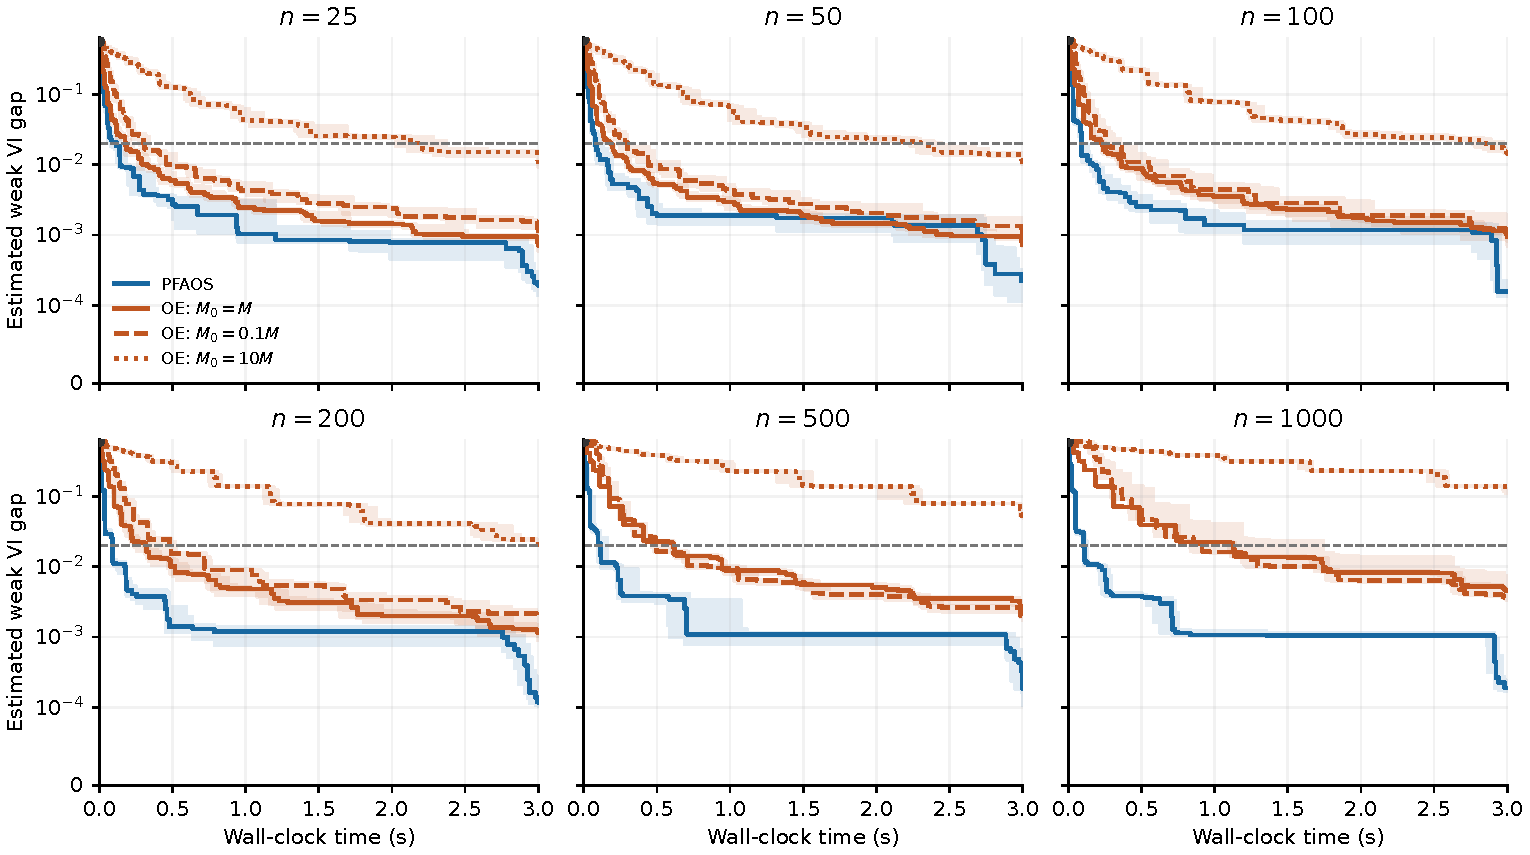
\includegraphics[width=0.97\linewidth]{results/figures/pfaos_residual.pdf}
\end{figure}

% Coupling-constraint violations: both methods remain at zero.
\begin{figure}[!htbp]
  \centering
  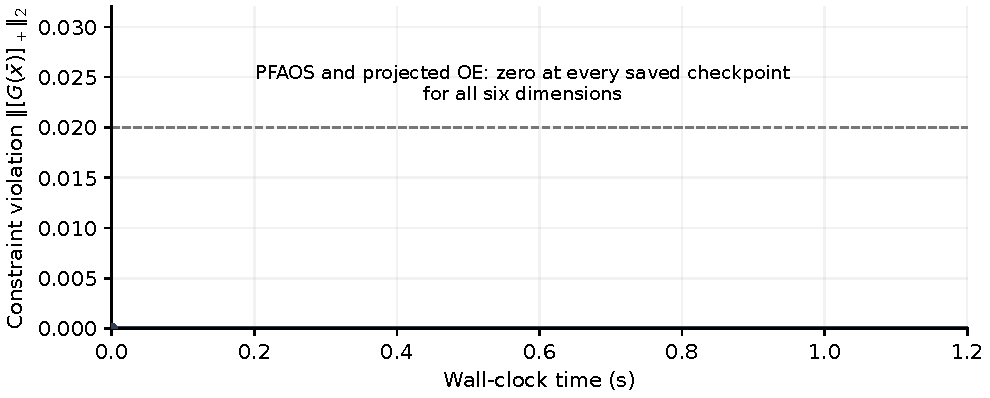
\includegraphics[width=0.92\linewidth]{results/figures/pfaos_violation.pdf}
\end{figure}

\begin{table}[!htbp]
\centering\scriptsize
\caption{PFAOS versus projected OE, varying dimension. Ten seeds per setting; numerical target $\varepsilon=0.02$. Times are wall-clock seconds, without normalization; normalization applies to the instances. Reached gives successful seeds/10. Time and work are medians over those seeds; final residuals use all ten. Gap estimates use numerical primal objectives, not certified upper bounds. FO/proj counts constraint-gradient calls for the proposed method, or generic projections for OE; dashes indicate no target crossing. OE labels specify the starting estimate $\widehat M_0\in\{M,0.1M,10M\}$; the operator line search is retained. All three are reported separately; no best-OE selection is used.}
\label{tab:pfaos_numerical}
\begin{tabular}{r l r r r r r}
\hline
$n$ & Method & Reached & Time (s) & $F$ calls & FO/proj & Final $\mathcal E$ \\
\hline
25 & PFAOS & 10/10 & 0.102 & 2,742 & 122 & 0.000193 \\
25 & Projected OE (M) & 10/10 & 0.181 & 28 & 27 & 0.000711 \\
25 & Projected OE (0.1M) & 10/10 & 0.305 & 46 & 45 & 0.00115 \\
25 & Projected OE (10M) & 10/10 & 2.17 & 316 & 315 & 0.0101 \\
\hline
50 & PFAOS & 10/10 & 0.0787 & 2,203 & 123 & 0.000223 \\
50 & Projected OE (M) & 10/10 & 0.181 & 28 & 27 & 0.000727 \\
50 & Projected OE (0.1M) & 10/10 & 0.29 & 39 & 38 & 0.00106 \\
50 & Projected OE (10M) & 10/10 & 2.35 & 316 & 315 & 0.011 \\
\hline
100 & PFAOS & 10/10 & 0.0894 & 2,404 & 123 & 0.000157 \\
100 & Projected OE (M) & 10/10 & 0.234 & 28 & 27 & 0.000943 \\
100 & Projected OE (0.1M) & 10/10 & 0.254 & 32 & 31 & 0.00112 \\
100 & Projected OE (10M) & 10/10 & 2.86 & 316 & 315 & 0.0145 \\
\hline
200 & PFAOS & 10/10 & 0.0879 & 2,096 & 123 & 0.000118 \\
200 & Projected OE (M) & 10/10 & 0.322 & 28 & 27 & 0.00116 \\
200 & Projected OE (0.1M) & 10/10 & 0.487 & 46 & 45 & 0.00181 \\
200 & Projected OE (10M) & 3/10 & 2.99 & 247 & 246 & 0.0208 \\
\hline
500 & PFAOS & 10/10 & 0.107 & 2,184 & 123 & 0.000186 \\
500 & Projected OE (M) & 10/10 & 0.616 & 28 & 27 & 0.00245 \\
500 & Projected OE (0.1M) & 10/10 & 0.493 & 22 & 21 & 0.00194 \\
500 & Projected OE (10M) & 0/10 & -- & -- & -- & 0.0515 \\
\hline
1000 & PFAOS & 10/10 & 0.108 & 2,039 & 124 & 0.000189 \\
1000 & Projected OE (M) & 10/10 & 1.13 & 28 & 27 & 0.00456 \\
1000 & Projected OE (0.1M) & 10/10 & 0.884 & 22 & 21 & 0.00348 \\
1000 & Projected OE (10M) & 0/10 & -- & -- & -- & 0.113 \\
\hline
\end{tabular}
\end{table}


PFAOS and OE initialized at either $M$ or $0.1M$ reach the target in
all ten seeds at every dimension. PFAOS has the lower median target time
throughout the grid, with medians between $0.079$ and $0.108$ seconds.
For OE initialized at $M$, the median increases from $0.181$ seconds at
$n=25$ to $1.131$ seconds at $n=1000$. At the latter dimension, OE
initialized at $0.1M$ requires a median of $0.884$ seconds, compared with
$0.108$ seconds for PFAOS. Thus a lower starting estimate can improve OE's
observed target time even after accounting for rejected line-search trials.
The acceptance test uses directional differences of $F$, so the global norm
$M$ need not give the fastest locally accepted steps.

The evaluation counts clarify this comparison. At $n=1000$, PFAOS uses
a median of $2039$ evaluations of $F$ and approximately $124$
constraint-gradient evaluations by the target checkpoint. OE initialized
at $M$ uses $28$ evaluations of $F$ and $27$ generic nonlinear projections;
starting at $0.1M$ gives $22$ evaluations of $F$ and $21$ projections,
including rejected trials. PFAOS performs substantially more operator work,
but its sparse evaluations and simple primal subproblems are sufficiently
inexpensive to yield the lower wall time. This illustrates the computational
tradeoff motivating operator sliding when full nonlinear projections are
costly.

The large overestimate has a more pronounced effect. At $n=25$, OE
initialized at $10M$ requires a median of $315$ projections and $2.169$
seconds to reach the target, compared with $27$ projections and $0.181$
seconds when initialized at $M$. The $10M$ configuration succeeds in all
ten seeds through $n=100$, in only three seeds at $n=200$, and in none
at $n=500$ or $1000$. Its conditional median at $n=200$ is $2.991$
seconds among the three successful runs. The operator line search only
increases its estimate, so it can correct an underestimate but does not
reduce an initially valid, conservative value such as $10M$.

At $n=1000$, the median final combined residuals under the common budget
are $1.89\times10^{-4}$ for PFAOS and $4.56\times10^{-3}$,
$3.48\times10^{-3}$, and $0.113$ for OE initialized at $M$, $0.1M$,
and $10M$, respectively. All saved single-constraint averages have zero
measured coupling-constraint violation in every configuration, so their
combined residuals coincide with their weak gaps. This observed feasibility
does not imply that PFAOS's affine models enforce the original quadratic
constraint at every iterate.

\subsubsection{MC-PFAOS versus projected OE.}
We first fix $n=50$ and vary the number of coupling constraints.
Table~\ref{tab:mc_pfaos_numerical} reports the complete constraint grid.
The accompanying figures show $m=100$, a setting at which both methods
reach the target in every seed. Each figure includes an early view and
a view of the full three-second run. The early windows cover the first
$0.02$ seconds for the weak gap and the first $0.12$ seconds for
constraint violation. In the table, ``FO/proj'' counts full Jacobian
evaluations for MC-PFAOS and generic nonlinear projections for OE;
$mN_J$ gives the corresponding number of component-gradient equivalents
for MC-PFAOS.

% MC-PFAOS versus projected OE: weak VI gap at n=50, m=100.
\begin{figure}[!htbp]
  \centering
  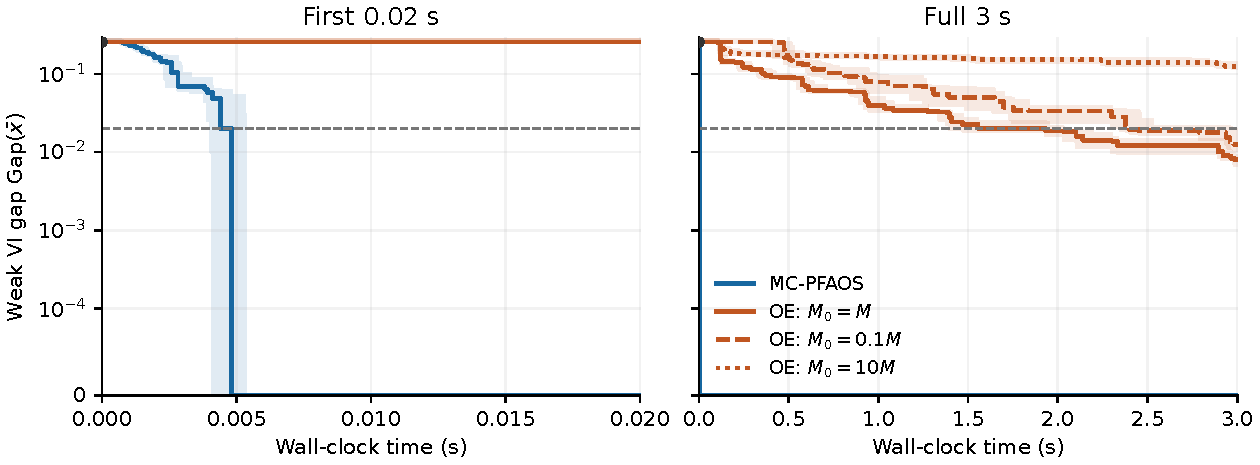
\includegraphics[width=0.92\linewidth]{results/figures/mc_residual.pdf}
\end{figure}

% The same runs' coupling-constraint violation.
\begin{figure}[!htbp]
  \centering
  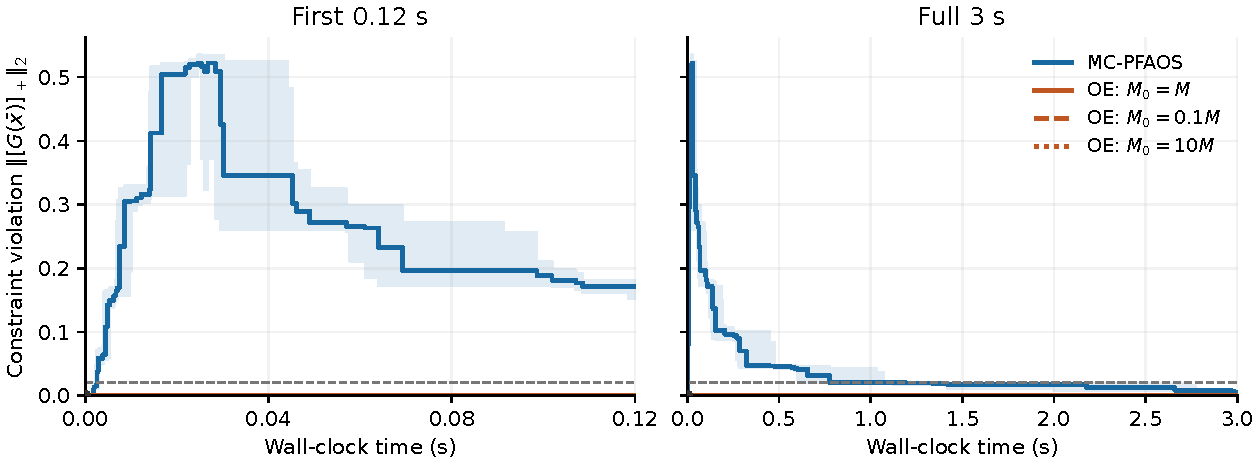
\includegraphics[width=0.92\linewidth]{results/figures/mc_violation.pdf}
\end{figure}

\begin{table}[!htbp]
\centering\scriptsize
\caption{MC-PFAOS versus projected OE, varying the number of constraints. Ten seeds per setting; target $\varepsilon=0.02$. Time and work are medians over successful runs; final residuals use all seeds. FO/proj counts full Jacobian calls and $mN_J$ counts individual component-gradient equivalents for the proposed method, or generic projections for OE; dashes indicate no target crossing.}
\label{tab:mc_pfaos_numerical}
\begin{tabular}{r l r r r r r r}
\hline
$m$ & Method & Reached & Time (s) & $F$ calls & FO/proj & $mN_J$ & Final $\mathcal E$ \\
\hline
2 & MC-PFAOS & 10/10 & 0.625 & 21,086 & 419 & 838 & 0.00315 \\
2 & Projected OE & 10/10 & 0.175 & 28 & 27 & -- & 0.000704 \\
\hline
5 & MC-PFAOS & 10/10 & 1.15 & 38,737 & 419 & 2,095 & 0.00363 \\
5 & Projected OE & 10/10 & 0.129 & 19 & 18 & -- & 0.000265 \\
\hline
10 & MC-PFAOS & 10/10 & 1.14 & 38,545 & 419 & 4,190 & 0.00404 \\
10 & Projected OE & 10/10 & 0.128 & 19 & 18 & -- & 0.000267 \\
\hline
20 & MC-PFAOS & 10/10 & 1.26 & 38,545 & 419 & 8,380 & 0.00402 \\
20 & Projected OE & 10/10 & 0.144 & 19 & 18 & -- & 0.000303 \\
\hline
40 & MC-PFAOS & 10/10 & 1.2 & 38,305 & 419 & 16,760 & 0.00416 \\
40 & Projected OE & 10/10 & 0.181 & 19 & 18 & -- & 0.000392 \\
\hline
100 & MC-PFAOS & 10/10 & 1.2 & 38,545 & 419 & 41,900 & 0.00401 \\
100 & Projected OE & 10/10 & 1.89 & 19 & 18 & -- & 0.00719 \\
\hline
250 & MC-PFAOS & 10/10 & 1.33 & 38,545 & 419 & 104,750 & 0.00465 \\
250 & Projected OE & 9/10 & 2.49 & 19 & 18 & -- & 0.0115 \\
\hline
500 & MC-PFAOS & 10/10 & 1.58 & 38,545 & 419 & 209,500 & 0.00541 \\
500 & Projected OE & 0/10 & -- & -- & -- & -- & 0.14 \\
\hline
\end{tabular}
\end{table}


With $\widehat M_0=M$ or $0.1M$, OE has the lower median target time
for every setting through $m=40$, and both configurations succeed in all
ten seeds. At $m=5$, the respective OE medians are $0.115$ and $0.182$
seconds, compared with $1.241$ seconds for MC-PFAOS. At $m=40$, they are
$0.166$ and $0.262$ seconds, compared with $1.209$ seconds for MC-PFAOS.
OE initialized at $10M$ also succeeds in every seed throughout this range,
but requires median times of $1.518$ and $1.931$ seconds at $m=5$ and
$40$. Its conservative operator estimate therefore changes the timing
comparison even when the projections involve relatively few constraints.

At $m=100$, MC-PFAOS reaches the target in all ten seeds with a median
time of $1.156$ seconds. OE initialized at $M$ also succeeds in all ten,
with a median of $1.742$ seconds. Starting at $0.1M$ gives eight successful
runs and a conditional median of $2.364$ seconds, whereas starting at
$10M$ gives no observed target crossing. At $m=250$, MC-PFAOS succeeds
in all ten seeds at a median of $1.314$ seconds. The corresponding success
fractions for OE are $9/10$, $5/10$, and $0/10$ for starting estimates
$M$, $0.1M$, and $10M$. The conditional medians for the two configurations
with successful runs are $2.140$ and $2.881$ seconds, respectively.

For $m=500$, MC-PFAOS again succeeds in all ten seeds, with a median
target time of $1.577$ seconds. None of the three OE configurations reaches
the target within the budget. The median final combined residual is
$5.76\times10^{-3}$ for MC-PFAOS, compared with $0.138$, $0.256$, and
$0.182$ for OE initialized at $M$, $0.1M$, and $10M$, respectively.
MC-PFAOS uses a median of $38{,}545$ operator evaluations and $419$
full Jacobian evaluations by the target checkpoint, corresponding to
$209{,}500$ component-gradient equivalents.

The same generic nonlinear projection is used in all three OE configurations.
The differences among them therefore arise from their initial operator
estimates and the resulting accepted steps and rejected trials. In
particular, correcting an underestimate requires additional full projections,
which can consume a substantial part of the budget when $m$ is large.
A large overestimate avoids these rejected trials but yields smaller steps,
and the line search does not reduce it. MC-PFAOS performs much more operator
work, while retaining simple primal and dual projections.

The constraint construction controls the scale of the problem as $m$
increases. The median initial weak gap is $0.261$ at $m=5$ and $0.256$
at $m=500$. The larger constraint sets nevertheless contain partly redundant
members of five resource families. The observed timing comparisons describe
this synthetic family and the specified fresh generic projection policy;
other constraint geometries or projection implementations can give different
results.

Table~\ref{tab:mc_dimension_numerical} reports the additional
dimension study at $m=5$. All four configurations reach the target in all ten
seeds for each dimension. For $n\in\{25,50,100\}$, OE's median target
times with $\widehat M_0=M$ are $0.115$, $0.115$, and $0.189$ seconds,
compared with $1.085$, $1.241$, and $0.945$ seconds for MC-PFAOS. Thus increasing
the dimension over this range, while retaining only five coupling
constraints, does not reverse OE's timing advantage.

\begin{table}[!htbp]
\centering\scriptsize
\caption{MC-PFAOS versus projected OE, varying dimension at $m=5$. Ten seeds per setting; target $\varepsilon=0.02$. Time and work are medians over successful runs; final residuals use all seeds. FO/proj counts full Jacobian calls and $mN_J$ counts individual component-gradient equivalents for the proposed method, or generic projections for OE; dashes indicate no target crossing.}
\label{tab:mc_dimension_numerical}
\begin{tabular}{r l r r r r r r}
\hline
$n$ & Method & Reached & Time (s) & $F$ calls & FO/proj & $mN_J$ & Final $\mathcal E$ \\
\hline
25 & MC-PFAOS & 10/10 & 0.971 & 35,140 & 523 & 2,615 & 0.00393 \\
25 & Projected OE & 10/10 & 0.107 & 19 & 18 & -- & 0.000228 \\
\hline
50 & MC-PFAOS & 10/10 & 1.15 & 38,737 & 419 & 2,095 & 0.00363 \\
50 & Projected OE & 10/10 & 0.129 & 19 & 18 & -- & 0.000265 \\
\hline
100 & MC-PFAOS & 10/10 & 0.889 & 29,508 & 523 & 2,615 & 0.00354 \\
100 & Projected OE & 10/10 & 0.149 & 19 & 18 & -- & 0.0004 \\
\hline
\end{tabular}
\end{table}


The separate plots also clarify the early behavior of MC-PFAOS. At
$n=50$ and $m=100$, its median weak gap decreases from $0.256$ at
initialization to $0.066$ at checkpoint $k=8$, while its median
constraint violation increases from zero to $0.058$. At checkpoint
$k=27$, the median weak gap is zero, but the median constraint violation
is $0.524$. A zero weak gap at this stage therefore does not indicate
attainment of the joint accuracy target. Subsequent primal and dual
updates reduce the violation sufficiently for every seed to reach the
target within the budget. This transient is consistent with the update
structure: MC-PFAOS projects its primal iterates onto $X$ and handles
the coupling constraints through dual variables, so its iterates and
reported averages need not satisfy all resource limits during the run.

Across the complete study, the weak gap is nonincreasing at every saved
MC-PFAOS checkpoint. This is an empirical observation; the convergence
bounds do not require the combined residual to decrease at every
checkpoint. Neither plotted component is replaced by a running minimum.
OE's saved averages have zero measured coupling-constraint violation.
The largest recorded norm of an outer dual iterate for MC-PFAOS is
approximately $2.81$; the dual updates use orthant projection and do
not truncate the multipliers at $\Lambda$.
